\documentclass[11pt,a4paper]{article}
\usepackage[utf8]{inputenc}
\usepackage[T1]{fontenc}
\usepackage[spanish,es-nodecimaldot]{babel}
\usepackage[margin=2.7cm]{geometry}
\usepackage{amsmath,amssymb,amsthm,mathtools}
\usepackage{graphicx,booktabs,tabularx,longtable,array,float}
\usepackage{natbib}
\usepackage{hyperref}
\hypersetup{hidelinks,pdfauthor={Brian Axel Rodriguez},pdftitle={La riqueza de la opcionalidad}}
\graphicspath{{../figures/}}
\setlength{\parindent}{1.1em}\setlength{\parskip}{0.18em}\setlength{\emergencystretch}{2em}
\newtheorem{theorem}{Teorema}[section]
\newtheorem{proposition}[theorem]{Proposición}
\newtheorem{corollary}[theorem]{Corolario}
\newtheorem{definition}[theorem]{Definición}
\newtheorem{assumption}[theorem]{Supuesto}
\newcommand{\E}{\mathbb E}\newcommand{\R}{\mathcal R}\newcommand{\Prb}{\mathbb P}\newcommand{\dd}{\mathrm d}\newcommand{\1}{\mathbf 1}\newcommand{\muF}{\mu_t}
\title{\textbf{La riqueza de la opcionalidad: liquidez, selección financiera y propagación de shocks en redes productivas}}
\author{Brian Axel Rodríguez\\\small Independent Research}
\date{2026}
\begin{document}\maketitle
\begin{abstract}
Una reserva líquida compra tiempo: permite sostener pagos, reorganizar insumos, esperar la cobranza o posponer una decisión irreversible. Este artículo desarrolla un marco teórico para estudiar cómo ese margen temporal puede afectar la selección de firmas y la propagación de perturbaciones en redes productivas. Primero, define el runway como recursos utilizables dentro del horizonte de obligaciones, sin equiparar cuentas por cobrar con caja ni confundir líneas comprometidas con crédito hipotético. Bajo una distribución Lomax explícita para shocks de caja, deriva la probabilidad de distress, su sensibilidad marginal y una medida de urgencia; la forma funcional es condicional a la distribución elegida y no se presenta como ley universal. Segundo, muestra cómo los atrasos de pago pueden reducir el runway efectivo y amplificar pérdidas a través de una red, bajo restricciones explícitas sobre monetización, sustitución y estabilidad del operador de propagación. Tercero, caracteriza cuándo una representación agregada por momentos es exacta y cuándo una aproximación por bins admite cotas de error. La condición de cierre por momentos exige que los estados omitidos —incluida la red y los pasivos fiscales o comerciales relevantes— no alteren la transición una vez fijados los agregados. Cuarto, audita la identificación empírica: la demora puede afectar la liquidez y la supervivencia, pero la fragilidad de la firma también puede alterar su puntualidad de pago, el acceso al crédito y la selección de proveedores. Los datos incluidos permiten describir ratios contables de emisoras argentinas; no observan simultáneamente facturas, fechas efectivas de pago, vínculos proveedor-cliente y salida de firmas. En consecuencia, no identifican causalmente el mecanismo. El aporte es una estructura analítica con resultados condicionales, condiciones de cierre verificables y una estrategia de contraste que distingue teoría, simulación y evidencia observacional.
\end{abstract}
\noindent\textbf{Palabras clave:} runway; liquidez; crédito comercial; selección de firmas; redes productivas; cierre micro--macro; endogeneidad.\\
\noindent\textbf{Clasificación JEL:} C63, D22, D85, E23, G32, L14, L25.

\section{Introducción}
Una empresa puede tener pedidos, trabajadores y tecnología productiva, pero no llegar al próximo período porque los salarios, los impuestos o los insumos vencen antes de que se cobren las ventas. La diferencia entre continuar operando y contraer la producción no tiene por qué coincidir con una diferencia de productividad. Puede depender del tiempo durante el cual la firma puede cubrir sus compromisos con recursos efectivamente accesibles. Ese margen temporal es el objeto económico que aquí denominamos \emph{runway}.

La idea no reemplaza las teorías de productividad, selección o redes. Las conecta mediante una restricción de liquidez de corto plazo. La literatura de gestión de liquidez subraya el valor precautorio de la caja cuando la financiación externa es costosa y el valor de los proyectos depende de la liquidez disponible en el futuro \citep{almeida2014,almeida2007,fazzari1988}. La literatura de redes productivas muestra que shocks idiosincráticos pueden propagarse a través de insumos específicos y vínculos de producción \citep{acemoglu2012,carvalho2014,barrot2016}. La literatura de crédito comercial demuestra que las obligaciones entre empresas pueden transmitir estrés financiero y que el crédito de proveedores funciona como una fuente de liquidez contingente \citep{boissay2013,jacobson2015,amberg2021,costello2020}. Estudios que combinan redes de producción y financiación encuentran que las restricciones financieras pueden amplificar shocks que se originan fuera de la firma afectada directamente \citep{demir2024,huremovic2026}. Estas contribuciones motivan el mecanismo, pero no demuestran que una misma parametrización describa cualquier economía ni que la demora pública sea exógena.

La contribución del artículo es deliberadamente delimitada. (i) Deriva una función de riesgo de liquidez y una medida de urgencia bajo una distribución de shocks explícita. (ii) establece condiciones bajo las cuales una demora de cobro reduce el runway y se transmite a otras firmas. (iii) formaliza la condición de cierre exacto por momentos y una cota de aproximación distribucional. (iv) distingue las afirmaciones que pueden probarse analíticamente de las que requieren cálculo numérico o datos microeconómicos. (v) examina endogeneidad, causalidad inversa, simultaneidad y efectos de red antes de formular una estrategia empírica.

El texto no presenta una bifurcación global, una histéresis general ni un efecto causal estimado. Los certificados numéricos asociados a un sistema reducido no se trasladan automáticamente a un campo derivado desde decisiones microeconómicas. Del mismo modo, un ejercicio sintético que reproduce una trayectoria no constituye calibración empírica. La tesis más modesta y defendible es que la liquidez puede alterar qué opciones productivas siguen siendo factibles, y que la fuerza de ese canal depende de la tecnología, las obligaciones, el crédito accesible y la topología de la red.

\section{Estado de la firma y contabilidad de liquidez}
Sea $i$ una firma activa en el período $t$. Denotemos por $C_{it}$ su caja disponible; $L^u_{it}$ el crédito comprometido y no dispuesto; $\theta_{it}\in[0,1]$ la fracción que puede utilizarse en el horizonte relevante; $F_{it}$ los fondos obtenidos por factoring u otra monetización efectiva, netos de cualquier activo que ya se haya contabilizado como cedido; $A^{g}_{it}$ las cuentas por cobrar al sector público aún no cobradas ni descontadas; $B_{it}>0$ el gasto imprescindible por unidad de tiempo; y $\omega_{it}\in[0,1]$ la fracción de las cuentas públicas que puede convertirse en liquidez dentro de ese horizonte.

Definimos el runway efectivo como
\begin{equation}
R_{it}=\frac{C_{it}+\theta_{it}L^u_{it}+F_{it}+\omega_{it}A^g_{it}}{B_{it}}. \label{eq:runway}
\end{equation}
La unidad de $R$ es tiempo si $B$ es gasto por unidad temporal. La expresión no implica que el valor nominal de una factura esté disponible: $\omega$ recoge únicamente su monetización factible antes del vencimiento de los compromisos considerados. Si una cuenta ya fue factorizada, debe excluirse de $A^g$ para evitar doble cómputo. Las líneas no comprometidas, el crédito que el banco podría otorgar en el futuro y las ventas esperadas tampoco forman parte del numerador sin una regla explícita de acceso.

La definición es un indicador de capacidad de pago de corto plazo, no una medida suficiente de solvencia ni una predicción automática de supervivencia. No incorpora por sí sola covenants, vencimientos discretos, concentración de clientes, garantías, costos de cierre, acceso a refinanciación, decisiones de propietarios o heterogeneidad en la secuencia temporal de cobros y pagos. En aplicaciones, estos componentes deben medirse o modelarse por separado.

La contabilidad de caja satisface una identidad stock--flujo de la forma
\begin{equation}
C_{i,t+1}=C_{it}+\text{Receipts}_{it}+\text{New credit}_{it}-\text{Payments}_{it}-\text{Debt service}_{it}-\text{Taxes}_{it}+\text{Other flows}_{it}. \label{eq:cashflow}
\end{equation}
Las cuentas por cobrar y por pagar se actualizan de forma consistente con los flujos realizados. Un aumento de cuentas por cobrar no es un ingreso de caja en el período de devengamiento; un aumento de cuentas por pagar es financiación comercial y una obligación futura, no ingreso operativo. La distinción importa porque un modelo puede producir un runway artificialmente creciente si acumula ventas devengadas como efectivo o si omite gastos de insumos, nómina, impuestos o reembolso de crédito.

\section{Del riesgo de caja a la urgencia}
\subsection{Definición general}
Sea $X_i\geq0$ la pérdida inesperada de caja acumulada durante el horizonte relevante. Si la reserva accesible es $B_iR_i$, el evento de distress de liquidez ocurre cuando $X_i>B_iR_i$. La probabilidad de distress es
\begin{equation}
q(R)=\Prb(X>BR)=1-F_X(BR),\qquad R\geq0. \label{eq:qgeneral}
\end{equation}
Si $X$ tiene densidad $f_X$ positiva en el rango pertinente, entonces $q'(R)=-Bf_X(BR)<0$. Esta propiedad no requiere escoger una distribución paramétrica. La distribución sí determina la forma de la cola, la velocidad de caída del riesgo y la extrapolación hacia niveles extremos de runway.

\subsection{Referencia Lomax y resultados analíticos}
Para obtener una forma cerrada, supóngase que el shock sigue una distribución Lomax de escala $s>0$ y forma $\alpha>0$, con función de supervivencia $\Prb(X>x)=(1+x/s)^{-\alpha}$. Entonces
\begin{equation}
q_L(R)=\left(1+\frac{BR}{s}\right)^{-\alpha}. \label{eq:lomax}
\end{equation}
La Lomax permite una cola de potencia y una representación parsimoniosa de pérdidas positivas con cola pesada. No se deduce de que $X$ sea positivo: es un supuesto que debe compararse con alternativas, entre ellas la lognormal, usando cuantiles extremos, ajuste fuera de muestra y estabilidad por sector y período.

\begin{proposition}[Urgencia bajo una cola Lomax]
Bajo la especificación de \eqref{eq:lomax}, la probabilidad de distress es decreciente y convexa en $R$. En particular,
\begin{align}
-q'_L(R)&=\frac{\alpha B}{s}\left(1+\frac{BR}{s}\right)^{-\alpha-1}, \label{eq:marginal}\\
q''_L(R)&=\frac{\alpha(\alpha+1)B^2}{s^2}\left(1+\frac{BR}{s}\right)^{-\alpha-2}>0. \label{eq:convex}
\end{align}
La elasticidad absoluta del riesgo respecto del runway es
\begin{equation}
\eta_L(R)=-\frac{R q'_L(R)}{q_L(R)}=\frac{\alpha BR}{s+BR}. \label{eq:elasticity}
\end{equation}
\end{proposition}
\begin{proof}
Derivar la función de supervivencia de \eqref{eq:lomax} una vez y dos veces produce \eqref{eq:marginal} y \eqref{eq:convex}. Multiplicar $-q'_L/q_L$ por $R$ simplifica a \eqref{eq:elasticity}. Los signos se siguen de $B,s,\alpha>0$.\end{proof}

Conviene distinguir tres objetos. $q(R)$ es una probabilidad; $-q'(R)$ mide la reducción marginal de esa probabilidad ante una unidad adicional de runway; $\eta(R)$ es una elasticidad. Una función objetivo podría penalizar el distress esperado, el costo de mantener caja o la pérdida marginal evitada, pero estas magnitudes no son intercambiables. Por ejemplo,
\begin{equation}
\mathcal C(R)=c_RR+c_Dq(R),\qquad c_R,c_D\geq0, \label{eq:cost}
\end{equation}
expresa un compromiso ilustrativo entre costo de mantener liquidez y costo esperado del distress. No es por sí sola una condición de equilibrio ni identifica los parámetros $c_R,c_D,s,\alpha$.

\begin{figure}[htbp]\centering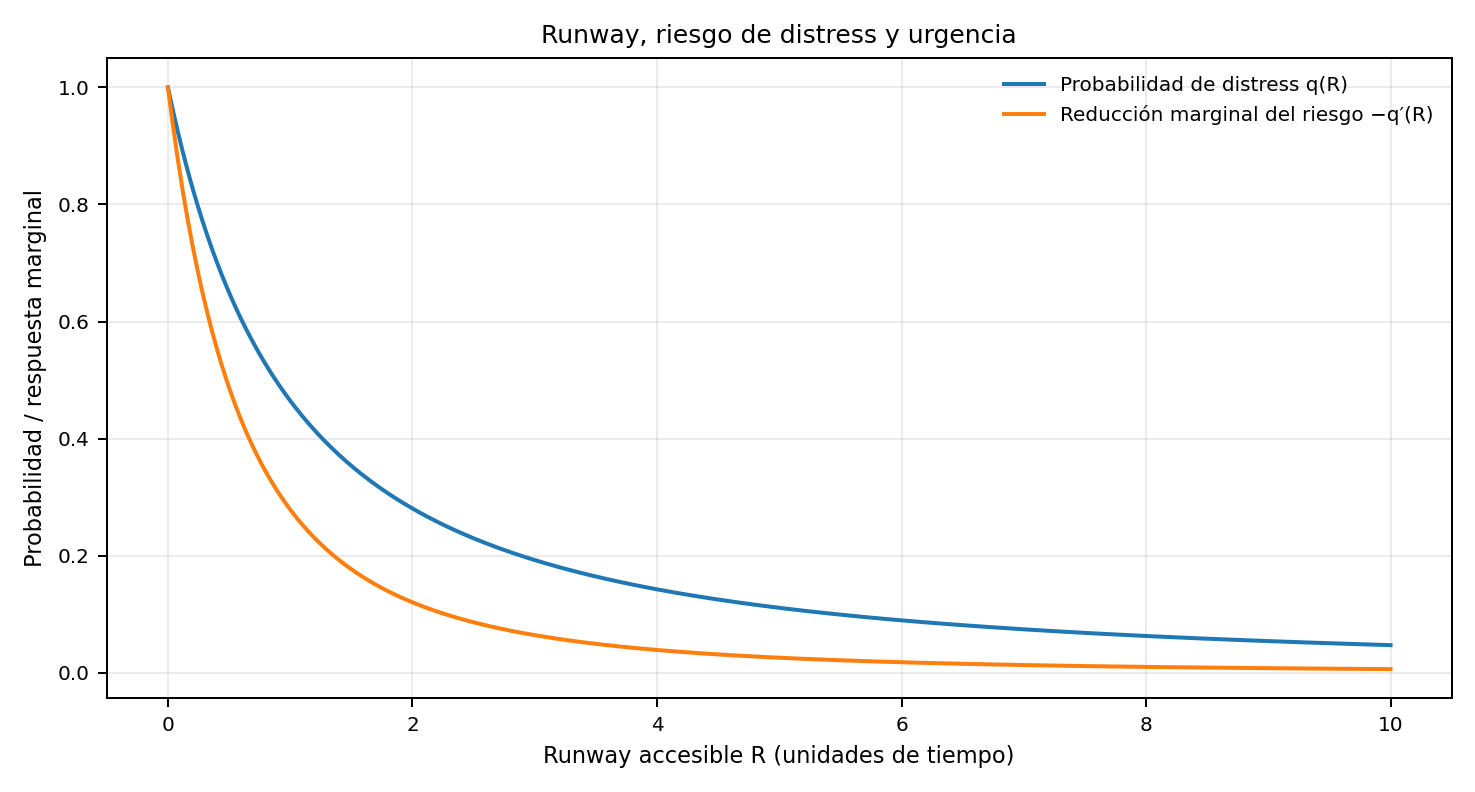
\includegraphics[width=.78\linewidth]{runway_urgency.png}\caption{Probabilidad de distress y reducción marginal del riesgo bajo una distribución Lomax. Los parámetros son ilustrativos, no estimados.}\label{fig:runway}\end{figure}

\section{Opcionalidad y decisión dinámica de la firma}
El runway es económicamente relevante porque modifica el conjunto de acciones que una firma puede financiar hasta el siguiente momento de ajuste. Sea $a\in\mathcal A$ una acción —continuar, invertir, innovar, sustituir un proveedor o esperar— y sea $c(a)$ su necesidad de caja en el horizonte. Para un estado con runway $R$, definimos el conjunto factible
\begin{equation}
\mathcal A(R)=\{a\in\mathcal A:c(a)\leq BR+M(a)\},
\end{equation}
donde $M(a)$ representa únicamente entradas o financiación verificablemente disponibles para esa acción. Si $R_2\geq R_1$ y las demás condiciones son iguales, entonces $\mathcal A(R_1)\subseteq\mathcal A(R_2)$. La liquidez puede ampliar el menú de decisiones aun cuando no modifique directamente la productividad tecnológica.

\begin{definition}[Valor de opcionalidad]
Sea $U(a,s)$ el valor de una acción $a$ en el estado $s$. El valor estático de la opcionalidad es $V(R,s)=\sup_{a\in\mathcal A(R)}U(a,s)$. La ganancia de opcionalidad entre dos niveles de runway es $\Omega(R_2,R_1;s)=V(R_2,s)-V(R_1,s)$ para $R_2\geq R_1$.
\end{definition}

\begin{proposition}[Monotonicidad de la opcionalidad]
Si el conjunto de acciones factibles es anidado en runway y los pagos de cada acción no cambian mecánicamente con $R$, entonces $V(R,s)$ es no decreciente en $R$ y $\Omega(R_2,R_1;s)\geq0$.
\end{proposition}
\begin{proof}
Como $\mathcal A(R_1)\subseteq\mathcal A(R_2)$, el supremo de $U(a,s)$ sobre el segundo conjunto no puede ser menor que el supremo sobre el primero.\end{proof}

En un problema dinámico, el valor de continuación puede escribirse como
\begin{equation}
V(s)=\max\left\{0,\sup_{a\in\mathcal A(R(s))}\left[u(s,a)+\beta\E\left(V(s')\mid s,a\right)\right]\right\}, \label{eq:bellman}
\end{equation}
donde la opción cero representa salida. La ecuación define el objeto, pero no lo resuelve: para obtener una solución se deben especificar estados, ley de movimiento, utilidad, restricciones de crédito, distribución de shocks y condición de frontera. La monotonía estática tampoco garantiza que aumentar la caja eleve la innovación realizada en todos los modelos. Una firma puede mantener efectivo, pagar deuda o distribuir dividendos; una opción disponible puede no elegirse; y el costo de financiar reservas puede cambiar junto con el runway. Por ello, el resultado de la proposición es una propiedad de factibilidad, no una predicción universal de inversión o productividad.

La conexión con la selección de firmas requiere separar productividad, liquidez y entrada. Los modelos clásicos de dinámica industrial muestran que heterogeneidad, aprendizaje, entrada y salida determinan la distribución de firmas de largo plazo \citep{jovanovic1982,hopenhayn1992}; en comercio, la reasignación entre firmas contribuye a la productividad agregada \citep{melitz2003}. La extensión aquí planteada es que la capacidad financiera puede cambiar qué firmas sobreviven a un shock y qué opciones conservan, condicional a su productividad. No se afirma que la liquidez reemplace la productividad ni que la selección financiera sea siempre dominante.

Para una población abierta, una representación general de la ley de movimiento es
\begin{equation}
\mu_{t+1}=\mathcal T(\mu_t;\vartheta_t)-\mathcal X(\mu_t;\vartheta_t)+\mathcal B(\mu_t;\vartheta_t),
\label{eq:openpopulation}
\end{equation}
donde $\mathcal T$ redistribuye la masa de firmas activas entre estados, $\mathcal X$ registra salidas y $\mathcal B$ entradas. La transición interna debe conservar masa; la masa activa cambia solo mediante flujos de entrada y salida. Esta contabilidad impide tratar la entrada como un apéndice sin interacción con la distribución existente. No obstante, escribir \eqref{eq:openpopulation} no prueba existencia de un equilibrio de largo plazo, unicidad de una distribución estacionaria ni histéresis. Esos resultados dependen de la regla de entrada, las ganancias esperadas, los costos hundidos, las transiciones de productividad y la red.

\subsection{Una microfundamentación mínima del valor de continuación}
Para que la ecuación de Bellman sea operativa, conviene separar el estado tecnológico del estado financiero. Sea $s=(z,R,d,g,a)$, donde $z$ denota productividad, $R$ runway efectivo, $d$ deuda neta, $g$ el estado de relaciones comerciales y $a$ edad o experiencia. La acción $u$ incluye producción, inversión, innovación, pagos comerciales y eventual salida. La transición es una distribución $P(\dd s'\mid s,u,\varepsilon)$, no una función determinista en general. El problema de una firma activa puede escribirse como
\begin{equation}
V(s)=\max\left\{V^{\mathrm{exit}}(s),\sup_{u\in\Gamma(s)}\left[\pi(s,u)-\chi(u)+\beta\int V(s')P(\dd s'\mid s,u)\right]\right\},
\label{eq:bellman_micro}
\end{equation}
donde $\Gamma(s)$ es el conjunto de acciones factibles, $\pi$ el flujo operativo neto, $\chi$ el costo de ajuste y $V^{\mathrm{exit}}$ el valor de liquidación neto de obligaciones. La restricción financiera debe entrar en $\Gamma(s)$ o en la transición de caja; no basta con incluir $R$ como covariable en una probabilidad de salida. En particular, si la acción exige un pago $m(u)$ antes de que se materialicen sus ingresos, una restricción mínima es $m(u)\leq C+\theta L^u+F+\omega A^g$, ajustada por obligaciones que vencen en el mismo horizonte.

Esta formulación es una plantilla de microfundamentación, no una solución computada del modelo. Para que defina un problema bien puesto se requieren: (i) un espacio de estados y acciones; (ii) una ley de transición para productividad, caja, deuda y contratos; (iii) una regla de precios o demanda; (iv) una convención de incumplimiento y liquidación; (v) una regla de entrada; y (vi) condiciones de integrabilidad que hagan finito el valor esperado. Sin esos elementos, no se puede invocar un teorema de contracción para afirmar existencia y unicidad de la función de valor.

\begin{proposition}[Monotonía del valor con inclusión de factibilidad]
Considérense dos estados que difieren solo en recursos líquidos, $s_1$ y $s_2$, con $R_2\geq R_1$. Si $\Gamma(s_1)\subseteq\Gamma(s_2)$, los pagos y las distribuciones de transición de cada acción común son iguales en ambos estados, y el valor de salida no disminuye, entonces $V(s_2)\geq V(s_1)$.
\end{proposition}
\begin{proof}
Bajo las hipótesis, cada acción factible en $s_1$ también es factible en $s_2$ y tiene el mismo valor de continuación. Por tanto, el supremo sobre $\Gamma(s_2)$ no es menor que el supremo sobre $\Gamma(s_1)$; la opción de salida tampoco reduce el máximo.\end{proof}

La hipótesis de transición idéntica es importante. Si la caja adicional genera costos de oportunidad, altera garantías, cambia el precio del crédito, induce una inversión irreversible o modifica las condiciones contractuales, los pagos o las transiciones dejan de ser iguales. En ese caso, la monotonía no se desprende de la inclusión de conjuntos factibles por sí sola. Tampoco implica que la caja observada sea exógena: las firmas con mejores oportunidades pueden acumular más caja y las firmas anticipando malos shocks pueden atesorarla.

\subsection{La entrada y la selección como condiciones de equilibrio}
La salida puede representarse mediante una regla de parada $\tau_e=\inf\{t:V^{\mathrm{continue}}(s_t)\leq V^{\mathrm{exit}}(s_t)\}$. Una entrada libre estilizada requiere que el valor esperado de entrar, neto del costo hundido $k_e$, no sea positivo en equilibrio:
\begin{equation}
\mathbb E[V(s_0)\mid \text{entrada}]-k_e\leq0,
\end{equation}
con igualdad si existe entrada interior. Esta condición no puede evaluarse sin especificar la distribución de estados de los entrantes y el efecto de la entrada sobre precios, demanda y red. Una regla computacional que repone aleatoriamente una fracción de las firmas que salen no equivale a entrada libre ni prueba una distribución estacionaria.

La ley de masa debe además distinguir firmas que sobreviven, nacimientos y firmas que salen. Para un conjunto medible $A$ de estados activos, una escritura contable es
\begin{equation}
\mu_{t+1}(A)=\int P(s,A\mid s,u^*(s),G_t)\,\mu_t(\dd s)+\nu_{t+1}(A)-\xi_{t+1}(A),
\label{eq:mass_balance}
\end{equation}
donde $\nu$ es la medida de entradas y $\xi$ la masa retirada. La identidad exige que la salida se reste solo de la masa que estaba activa y que los entrantes no se cuenten como supervivientes del período anterior. La estacionariedad requeriría $\mu_{t+1}=\mu_t$ junto con consistencia de entrada, precios y red; no se deduce de una población acotada por construcción.

\subsection{Qué significa cerrar el modelo micro--macro}
El cierre no se obtiene al elegir unos pocos momentos y simular sus transiciones. Sea $S(\mu,G,\ell)$ el vector de agregados y estados auxiliares. Para una transición completa $\mathcal T$, el cierre exacto exige que dos microestados con los mismos agregados produzcan los mismos agregados siguientes. Equivalentemente, para todo par $x_1,x_2$ tal que $S(x_1)=S(x_2)$ debe cumplirse
\begin{equation}
S(\mathcal T(x_1))=S(\mathcal T(x_2)).
\label{eq:fiber_test}
\end{equation}
La condición es falsable: se pueden construir microestados con igual caja media, productividad media y masa activa, pero diferente dispersión de runway, concentración de clientes o distribución de vencimientos. Si sus siguientes agregados difieren, el conjunto de momentos elegido no cierra el sistema. La red no puede omitirse cuando la transición depende de exposiciones que no son función de los agregados incluidos; tampoco puede resumirse por grado medio si el resultado depende de centralidad, dirección de flujos o correlación entre fragilidad y posición de red.

Una aproximación por bins constituye un paso numérico posterior, no una prueba de cierre. Deben reportarse por separado: (a) error de representación de la distribución dentro de cada bin; (b) error del campo agregado inducido por la proyección; (c) error de integración temporal; y (d) error de aproximación de la red. La cota de Grönwall controla solo el error de trayectoria una vez que existe una cota uniforme del campo y una constante de Lipschitz válida en una región invariante común. Si el estado discreto cambia, la salida crea discontinuidades o la red se rewirea, esos supuestos requieren demostración adicional.

\subsection{Cierre distribucional frente a cierre por momentos finitos}
Una afirmación precisa de cierre debe especificar el nivel de agregación. Sea el estado completo de la firma
\[
x_i=(c_i,d_i,\ell_i,r_i,\mathbf a_i,z_i,k_i,n_i,\tau_i),
\]
donde las coordenadas registran caja, deuda, crédito utilizable, inventarios, el vector de cuentas por cobrar/pagar por vencimiento, productividad, capacidad productiva, requerimientos de insumos y estado contractual/de pagos. Sea $G_t$ la red dirigida y ponderada de proveedores, y sea $\mathfrak M_t=(N_t,(x_i)_{i\leq N_t},G_t,\ell_t^A)$ el estado completo de población, red y variables agregadas de precios o fiscales que requieran las decisiones individuales. Se conserva deliberadamente la red etiquetada completa: la distribución marginal de estados de firma no preserva en general quién comercia con quién.

\begin{assumption}[Suficiencia de estado Markoviano]
Condicional al estado completo $\mathfrak M_t$, la ley de shocks exógenos está especificada; la regla de decisión de cada firma activa depende solo de su estado y del estado agregado/de red incluido; están especificados los núcleos de entrada y salida; y la actualización de la red y de los precios agregados sigue núcleos de transición especificados. Ninguna variable histórica omitida afecta esas leyes condicionales.
\end{assumption}

\begin{theorem}[Cierre micro--macro distribucional]
Bajo la suficiencia de estado Markoviano existe un núcleo de transición $\mathcal P$ tal que
\[
\Pr(\mathfrak M_{t+1}\in A\mid\mathfrak M_0,\ldots,\mathfrak M_t)=\mathcal P(A\mid\mathfrak M_t)
\]
para todo conjunto medible $A$. Por tanto, el estado completo de población y red es Markoviano y cierra exactamente en distribución. El resultado no implica que un vector finito de momentos, ni la distribución de runway por sí sola, sea un estado suficiente.
\end{theorem}

\begin{proof}[Esbozo de demostración]
Por hipótesis, condicionados al estado completo actual, las decisiones, los shocks idiosincráticos, los eventos de entrada/salida, la actualización de red y la actualización del estado agregado tienen leyes condicionales especificadas que no dependen de la historia anterior. Su ley condicional conjunta determina entonces la distribución del siguiente estado completo como función de $\mathfrak M_t$ solamente. Integrar sobre los shocks especificados produce el núcleo $\mathcal P$. Si un vencimiento, inventario, contrato, precio o variable histórica de red omitida altera alguna de esas leyes, la hipótesis falla y el estado propuesto no cierra.
\end{proof}

Este teorema establece un cierre micro--macro en el nivel distribucional del estado completo, no un equilibrio resuelto ni una reducción finito-dimensional. También identifica la carga de prueba para una agregación más pequeña: debe demostrarse que las fibras del mapa agregado son invariantes respecto de la ley de los agregados del período siguiente. El ABM actual cierra solo su sistema de reglas programadas; todavía no contiene los inventarios, la tecnología de insumos complementarios, los precios endógenos y los estados contractuales más ricos necesarios para afirmar el cierre completo del mecanismo económico.

\subsection{Prueba de consistencia del laboratorio basado en agentes}
El simulador se revisó para que los insumos del período deban financiarse antes de producir y las ventas realizadas se escalen por la proporción de insumos planeados que efectivamente se compró. Esto elimina la inconsistencia lógica previa, por la cual el racionamiento afectaba la salida pero no las ventas contemporáneas. La relación proporcional sigue siendo una restricción de cantidad estilizada, no una tecnología productiva estimada: inventarios, múltiples insumos complementarios, utilización de capacidad y precios endógenos de insumos no están modelados por completo. Por eso, el ABM es un laboratorio de mecanismos, no un modelo de red productiva calibrado, y sus resultados no identifican una elasticidad causal de productividad respecto de la demora.

La auditoría pendiente debe probar identidades de caja y deuda por período, conservación de flujos entre compradores y proveedores, casos límite (demora cero, ausencia de canal público, red vacía, crédito abundante y ausencia de shocks), sensibilidad global y momentos fuera de muestra. La calibración dinámica sigue sin ser satisfactoria y solo debe reconsiderarse después de verificar esas identidades y reglas de transición; de lo contrario, el ajuste de parámetros confundiría una mala especificación estructural con un problema paramétrico.

\subsection{Alternativa lognormal y robustez funcional}
Una especificación alternativa emplea una cola lognormal. Si $\ln X\sim N(m,\sigma^2)$, con $R>0$, defínase $z(R)=[\ln(BR)-m]/\sigma$. Entonces
\begin{equation}
q_{LN}(R)=\overline\Phi(z(R)),\qquad -q'_{LN}(R)=\frac{\phi(z(R))}{\sigma R},\qquad -\frac{Rq'_{LN}(R)}{q_{LN}(R)}=\frac{\phi(z(R))}{\sigma\overline\Phi(z(R))}. \label{eq:lognormal}
\end{equation}
La última expresión es la razón inversa de Mills, escalada por $1/\sigma$. A diferencia de la Lomax, la lognormal no impone una cola de potencia. Ninguna de las dos distribuciones queda identificada por la positividad de los shocks; su elección debe basarse en el ajuste de la cola, la estabilidad fuera de muestra y la relevancia económica del horizonte de riesgo. Por ello, los resultados cerrados anteriores son comparativas estáticas condicionales, no una afirmación sobre la distribución universal de pérdidas empresariales.

\section{Demoras de pago y propagación en redes}
\subsection{Efecto directo sobre runway}
Supóngase que la demora de pago público es $\tau$ y que la monetización oportuna de facturas satisface $\omega'(\tau)\leq0$. Manteniendo constantes los demás componentes de \eqref{eq:runway},
\begin{equation}
\frac{\partial R_i}{\partial\tau}=\frac{A_i^g}{B_i}\omega'_i(\tau)\leq0. \label{eq:dRdtau}
\end{equation}
Defínase $h_i(R)=h_0+\kappa q(R)$ con $h_0,\kappa\geq0$ y $h_0+\kappa\leq1$. Como $0<q(R)\leq1$, esta restricción garantiza $h_i(R)\in[0,1]$ para todo $R\geq0$. Entonces $\partial h_i/\partial\tau=\kappa q'(R_i)\partial R_i/\partial\tau\geq0$. El signo es una implicación condicional de la definición de exposición, no una estimación empírica. Puede desaparecer si la factura se descuenta plenamente, el gasto no vence antes del cobro, el proveedor sustituye al comprador o la demora coincide con otras entradas de caja compensatorias.

\begin{proposition}[Comparativa estática de la demora]
Si $A_i^g/B_i\geq0$, $\omega_i'(\tau)\leq0$, $q'(R)<0$, $h_0,\kappa\geq0$ y $h_0+\kappa\leq1$, entonces una mayor demora no aumenta el runway y no reduce el hazard de salida: $\partial R_i/\partial\tau\leq0$ y $\partial h_i/\partial\tau\geq0$.
\end{proposition}
\begin{proof}
La primera desigualdad se obtiene de \eqref{eq:dRdtau}. Para la segunda, aplicar la regla de la cadena al hazard y multiplicar dos derivadas no positivas: $\kappa q'(R_i)\partial R_i/\partial\tau\geq0$.\end{proof}

\subsection{Red de proveedores y estabilidad de la propagación}
Sea $W$ una matriz no negativa de exposición en la red de pagos, donde $W_{ij}$ es la participación de las ventas de la firma proveedora $i$ que corresponde al cliente $j$. Sea $u\geq0$ el vector de pérdidas directas de liquidez. Una aproximación lineal local al efecto de rondas sucesivas de transmisión puede escribirse como
\begin{equation}
x=u+\beta Wx,\qquad x=(I-\beta W)^{-1}u, \label{eq:network}
\end{equation}
si el radio espectral satisface $\rho(\beta W)<1$. Bajo esta condición, la serie de Neumann converge y
\begin{equation}
x=\sum_{k=0}^{\infty}(\beta W)^ku\geq u. \label{eq:neumann}
\end{equation}
La desigualdad es componente a componente y se sigue de la no negatividad de $W$. La inversa es un \emph{multiplicador de equilibrio de corto plazo con red congelada}: mantiene fijos el conjunto de firmas activas, la matriz de exposición y el coeficiente de respuesta local, antes de que se activen umbrales de salida, sustitución de proveedores o renegociación contractual. Muestra cómo una pérdida directa puede generar rondas adicionales dentro de ese régimen local; no dice que toda firma sufra el mismo efecto ni que el multiplicador lineal sea válido cuando las firmas salen, cambian proveedores o alteran endógenamente sus contratos.

La sustituibilidad reduce la exposición efectiva. Una parametrización ilustrativa es $\widetilde W_{ij}=W_{ij}(1-\sigma_{ij})$, con $\sigma_{ij}\in[0,1]$. Sin datos sobre sustitución, concentración de compras y enlaces comerciales, $\sigma$ no se identifica a partir de balances agregados. La matriz de exposición debe construirse con relaciones previas al shock si se utiliza para identificar spillovers; la red contemporánea puede ser consecuencia del propio estrés.

\subsection{Restricción de capital de trabajo y producción realizada}
Una forma mínima de vincular caja con producción consiste en separar producción potencial de producción realizada. Sea $y_i^*=A_i k_i^{\alpha}l_i^{\gamma}$ la producción potencial, con $\alpha,\gamma\geq0$ y $\alpha+\gamma\leq1$. Si el proceso requiere un insumo intermedio $m_i$ por unidad de producto, la restricción física es $y_i\leq m_i/\nu_i$, donde $\nu_i>0$ es el requerimiento unitario. Si además la compra del insumo debe pagarse antes de vender, el presupuesto líquido limita $m_i$:
\begin{equation}
 m_i\leq \frac{C_i+\theta_iL_i^u+F_i+\omega_iA_i^g-\mathcal O_i}{p_i^m},\qquad
 y_i=\min\left\{y_i^*,\frac{m_i}{\nu_i}\right\},
\label{eq:working_capital_prod}
\end{equation}
donde $\mathcal O_i$ son otras obligaciones que vencen antes de la venta y $p_i^m$ es el precio del insumo. La forma es ilustrativa: con varios insumos complementarios, la restricción relevante es el mínimo sobre todos los insumos necesarios; con inventarios, crédito de proveedor o pagos parciales, se requiere una transición intertemporal más rica.

La ecuación muestra por qué no debe identificarse productividad con ventas observadas. Una caída de $y_i$ puede surgir de menor $A_i$, de menos capital o trabajo, o de un insumo que no pudo financiarse. A su vez, las ventas nominales mezclan cantidades y precios. Medir la productividad de una firma requiere producción e insumos reales, tratamiento de márgenes y utilización de capacidad y atención a la selección por salida; aquí no se dispone de ese panel enlazado.

El mecanismo de red puede incorporarse haciendo que la disponibilidad de $m_i$ dependa de entregas de proveedores $j$, que a su vez dependen de sus propias restricciones de caja. La transición pasa entonces a ser simultánea o secuencial según el calendario de producción, entrega y pago. Si las entregas se determinan antes de las ventas, la restricción de capital de trabajo puede generar un efecto de cantidad; si los proveedores entregan a crédito, el canal inmediato puede operar sobre cuentas por pagar antes de afectar producción. La elección del orden temporal no es un detalle de programación: determina qué shocks se propagan en el mismo período y cuáles con rezago.

\section{Distribución de firmas, cierre y aproximación por bins}
\subsection{Ley distribucional}
Sea $s$ el estado de la firma y $G$ el grafo de relaciones comerciales. Denotemos por $\mu_t$ la medida de masa sobre estados activos y por $T_t$ el operador de transición que combina decisiones, shocks, cambio de rutina, entrada y salida. La ley exacta conjunta de la población y la red es $(\mu_{t+1}, G_{t+1}) = T_t(\mu_t, G_t)$. Los agregados observables se obtienen mediante un mapa $S(\mu_t,G_t,\ell_t)$ que puede incluir masa activa, distribución de runway, productividad, deuda, cuentas por pagar y estructura de red.

\begin{definition}[Cierre exacto por momentos]
El sistema agregado cierra exactamente respecto de $S$ si existe un operador $\Phi$ tal que $S(T(\mu, G)) = \Phi(S(\mu, G))$ para todos los estados admisibles y configuraciones topológicas, incorporando de manera nativa la red posterior generada por la transición económica.
\end{definition}

\begin{theorem}[Condición necesaria y suficiente de cierre]
Para una transición conjunta $T$ y un mapa agregado $S$, existe una función $\Phi$ que satisface $S(T(\mu, G)) = \Phi(S(\mu, G))$ en el dominio si y solo si $S(T(\mu_1, G_1)) = S(T(\mu_2, G_2))$ siempre que $S(\mu_1, G_1) = S(\mu_2, G_2)$. Es decir, la aplicación $S \circ T$ debe ser constante en cada fibra de $S$.
\end{theorem}
\begin{proof}
Si existe $\Phi$, dos configuraciones microeconómicas de población y red $(\mu_1, G_1)$ y $(\mu_2, G_2)$ con el mismo valor agregado $S$ tienen la misma imagen bajo $S \circ T$ por sustitución directa. A la inversa, si $S \circ T$ es constante en cada fibra, defínase $\Phi(s)$ como $S(T(\mu, G))$ para cualquier par $(\mu, G)$ tal que $S(\mu, G) = s$. Esta condición garantiza que la definición es estrictamente independiente del representante topológico seleccionado de la fibra.
\end{proof}

La consecuencia económica es importante: la distribución marginal del runway no basta como estado agregado si dos firmas con el mismo runway enfrentan contratos, proveedores, pasivos o posibilidades de sustitución diferentes que alteran sus transiciones. El estado mínimo debe incluir las variables que modifican las decisiones futuras. Este requisito es consistente con la literatura de heterogeneidad y agregación, donde el cierre por pocos momentos es una propiedad de una clase de modelos, no una identidad universal \citep{krusell1998,achdou2022}.

\subsection{Cota de proyección}
Supóngase que el integrando $f$ es Lipschitz en runway con constante $L_f$ y que cada bin $B_k$ tiene diámetro no mayor que $\Delta$. Para una medida de probabilidad $\mu$ y un representante $r_k\in B_k$, la aproximación es $\widehat I=\sum_k f(r_k)\mu(B_k)$.
\begin{proposition}[Error de integración por bins]
Bajo los supuestos anteriores,
\begin{equation}
\left|\int f(R)\,\dd\mu(R)-\sum_k f(r_k)\mu(B_k)\right|\leq\frac{L_f\Delta}{2}, \label{eq:binbound}
\end{equation}
si $r_k$ es el punto medio de cada bin.
\end{proposition}
\begin{proof}
Para todo $R\in B_k$, $|f(R)-f(r_k)|\leq L_f|R-r_k|\leq L_f\Delta/2$. Integrar en cada bin, sumar y usar $\sum_k\mu(B_k)=1$ produce la cota.\end{proof}

La cota de integración no es una cota del error del campo dinámico. Para aproximar trayectorias, supóngase adicionalmente que los campos $F$ y $F_K$ son Lipschitz con constante común $L$ en una región invariante y que $\sup_x\|F(x)-F_K(x)\|\leq\delta_K$. Si $x(0)$ y $x_K(0)$ son estados iniciales, Grönwall implica
\begin{equation}
\|x(t)-x_K(t)\|\leq e^{Lt}\|x(0)-x_K(0)\|+\frac{\delta_K}{L}(e^{Lt}-1),\quad L>0. \label{eq:gronwall}
\end{equation}
La cota solo es válida en un régimen local donde el conjunto de firmas activas permanece estable durante la ventana temporal acotada; la salida discreta de firmas o el rewiring puede volver discontinuo al campo vectorial o hacerlo solo Lipschitz por tramos. La demostración parte de la desigualdad integral para la diferencia de trayectorias y aplica la desigualdad de Grönwall. La expresión requiere una cota del campo, una región común y regularidad Lipschitz; no convierte automáticamente un algoritmo de bins en una aproximación certificada. Tampoco certifica raíces estacionarias, estabilidad, pliegues o histéresis. Para eso hacen falta errores de campo y jacobiano, búsqueda de ramas y, cuando se afirme existencia rigurosa, verificación intervalar del sistema específico.

\subsection{Heterogeneidad: por qué el runway medio no basta}
La distribución de runway importa incluso si el único resultado de interés es el distress esperado. Bajo la referencia Lomax y un gasto $B$ común, $q_L(R)=(1+BR/s)^{-\alpha}$ es estrictamente convexa para $R\geq0$, porque
\begin{equation}
q_L''(R)=\alpha(\alpha+1)\left(\frac{B}{s}\right)^2\left(1+\frac{BR}{s}\right)^{-\alpha-2}>0.
\end{equation}
Por la desigualdad de Jensen, para una distribución de runway con media finita,
\begin{equation}
\mathbb E[q_L(R)]\geq q_L(\mathbb E[R]),
\label{eq:jensen_distress}
\end{equation}
con desigualdad estricta si el runway no es degenerado. Por tanto, sustituir una distribución heterogénea por su media subestima el distress esperado bajo esta especificación. La diferencia no es un efecto causal de la desigualdad financiera: es una implicación matemática de la curvatura de la función de riesgo. Con gasto heterogéneo $B_i$, la desigualdad no se aplica directamente a la media de $R_i$; debe calcularse la distribución conjunta de $B_iR_i$ o del cociente de reservas y obligaciones.

La composición de la distribución también importa. Una transferencia de caja desde una firma con runway alto hacia una firma con runway bajo puede reducir la suma de riesgos si las ganancias marginales de reducir distress son mayores en la firma receptora y no existen costos de transferencia. Sin embargo, la afirmación depende de que las reservas se midan sobre el mismo horizonte y de que los fondos puedan reasignarse sin fricciones. En la práctica, caja atrapada en una subsidiaria, garantías específicas, restricciones regulatorias o compromisos de acreedores pueden impedir esa transferencia. El resultado de Jensen justifica conservar dispersión y colas en el estado agregado; no prescribe una política de redistribución sin modelar restricciones.

Una descomposición empírica útil debe reportar media, mediana, cuantiles bajos, masa cercana a cero y heterogeneidad por sector y tamaño, además de ratios agregados. Las firmas con caja alta pueden tener simultáneamente obligaciones próximas altas, por lo que un promedio de caja por activo no equivale al promedio de runway. El indicador debe usar partidas coherentes de numerador y denominador y evitar promediar cocientes sin mostrar el denominador. Estas decisiones afectan tanto la calibración como la interpretación de los momentos usados en inferencia indirecta.

\section{Inferencia indirecta y contenido informativo de los momentos}
Si se dispone de datos de firmas y de un simulador completamente especificado, la inferencia indirecta puede estimar parámetros estructurales $\vartheta$ comparando momentos observados con los generados por el modelo \citep{gourieroux1993}. Sea $m_D$ el vector de momentos de los datos y $m_S(\vartheta)$ el vector de momentos simulados. Un estimador de distancia es
\begin{equation}
\widehat\vartheta=\arg\min_{\vartheta\in\Theta}[m_D-m_S(\vartheta)]'W[m_D-m_S(\vartheta)],\qquad W\succeq0. \label{eq:indirect}
\end{equation}
La fórmula no produce identificación por sí sola. Los momentos deben tener una relación diferenciada con los parámetros, y el jacobiano $J(\vartheta)=\partial m_S(\vartheta)/\partial\vartheta'$ debe tener rango columna completo en el entorno relevante para la identificación local regular. Si dos parámetros desplazan los mismos momentos de forma similar, la función objetivo puede tener un valle plano y la estimación será débilmente identificada.

La elección de momentos debe corresponder a los canales teóricos. Los cuantiles de runway informan sobre la distribución de recursos accesibles y gastos; la frecuencia y duración de atrasos informan sobre el proceso de pago; la relación entre shocks directos y pérdidas de proveedores informa sobre la propagación de red; y la salida condicionada por productividad y liquidez informa sobre selección. Los momentos agregados de PIB o PTF no sustituyen a los momentos de pagos y redes, porque no separan esos canales. DSO y DPO pueden ayudar a describir capital de trabajo, pero no equivalen a fechas de vencimiento y pago realizadas.

La inferencia indirecta debe incorporar incertidumbre muestral, error de medición y variación entre semillas. Debe además evaluarse con momentos no utilizados en el ajuste y con períodos o firmas retenidos. Recuperar parámetros conocidos en datos sintéticos verifica que el algoritmo puede funcionar bajo el proceso generador especificado; no demuestra que los mismos parámetros estén identificados en los datos reales. En el estado actual, la fórmula se presenta como protocolo y no como estimación estructural ejecutada.

\section{Límites de los datos públicos y diagnóstico de las bases disponibles}
El piloto contable procedente de Yahoo Finance contiene 537 informes de 52 emisoras argentinas entre octubre de 2021 y agosto de 2026. El archivo consolidado supuestamente multi-país fue auditado y resultó estructuralmente idéntico al archivo de Argentina; por eso se descartó como muestra internacional y el análisis se limita al piloto descriptivo de 52 emisoras argentinas. Hay 240 filas anuales y 297 trimestrales, con superposición temporal; las observaciones trimestrales se concentran en 2025--2026 y parte de 2026 es incompleta. No corresponde apilar ambas frecuencias como observaciones independientes.

En la muestra anual no financiera, el archivo auditado incluye 173 observaciones válidas de runway estricto: mediana 25,37 días, percentil 10 de 4,43 y percentil 90 de 93,49. La mediana de DSO es 36,89 días y la de DPO 61,80 días. Son estadísticas por fila, no ponderadas por empresa. El panel no es representativo de las firmas no cotizadas y excluye empresas que ya salieron. El DPO contiene alertas de mapeo de partidas; los valores extremos requieren volver a la fuente, no borrado automático. La medida de runway tampoco incorpora automáticamente líneas comprometidas, calendario de vencimientos, cobros futuros ni pagos no operativos.

El piloto no observa identificadores de factura, fecha contractual de vencimiento, fecha efectiva de pago, comprador o proveedor, contratos públicos, ni salida real. Por tanto, no permite medir una exposición predeterminada a atrasos públicos ni reconstruir spillovers. La encuesta WBES puede describir establecimientos y preguntas sobre contratos o pagos públicos, sujeto a cuestionario, diseño muestral y pesos; una tabla pública de frecuencias no equivale a microdatos listos para estimación. No se reporta aquí una regresión microeconómica con esos datos.

Además, el catálogo y la tabla pública de frecuencias de la World Bank Enterprise Survey de Argentina permiten describir preguntas sobre contratos públicos y plazos de cobro. La documentación consultada reporta 797 establecimientos en el catálogo; 111 con contrato público reciente (J.42) y 108 respuestas numéricas para días hasta recibir pagos bajo esos contratos (J.43). La media no ponderada es 62,7 días, la mediana 60 y el percentil 90 109,5; el 22,2\% de las respuestas numéricas registra al menos 90 días, con máximo de 300. Estos valores proceden de frecuencias públicas, no de una regresión con microdatos descargados, y no deben interpretarse como una estimación causal ni como representatividad verificada sin revisar pesos, diseño muestral y códigos especiales \citep{wbes2026}.

\begin{table}[htbp]\centering\small
\caption{Pagos bajo contratos públicos en la tabla de frecuencias de WBES Argentina}
\begin{tabular}{lr}\toprule
Indicador & Valor \\\midrule
Establecimientos en el catálogo & 797 \\
Con contrato público reciente (J.42) & 111 \\
Respuestas numéricas de J.43 & 108 \\
Media no ponderada de días & 62,7 \\
Mediana de días & 60 \\
Percentil 90 de días & 109,5 \\
Respuestas con al menos 90 días & 22,2\% \\
Máximo observado en la tabla de frecuencias & 300 \\\bottomrule
\end{tabular}
\end{table}

\begin{figure}[htbp]\centering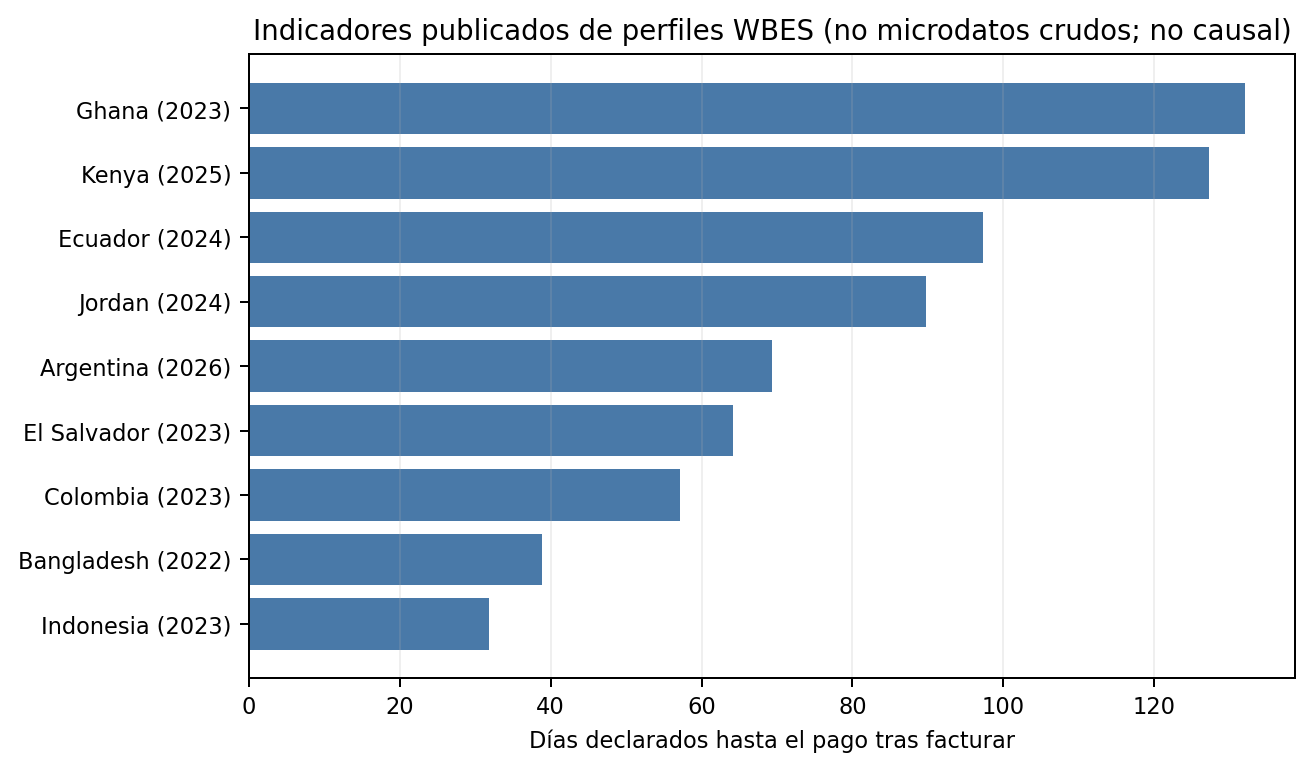
\includegraphics[width=.78\linewidth]{Fig10_WBES_payment_lags_ES.png}\caption{Distribución de frecuencias pública de los plazos de pago declarados para contratos públicos en la encuesta de Argentina. La figura es descriptiva; no es una estimación con microdatos ponderados ni una estimación causal.}\label{fig:wbeslags}\end{figure}

\begin{figure}[htbp]\centering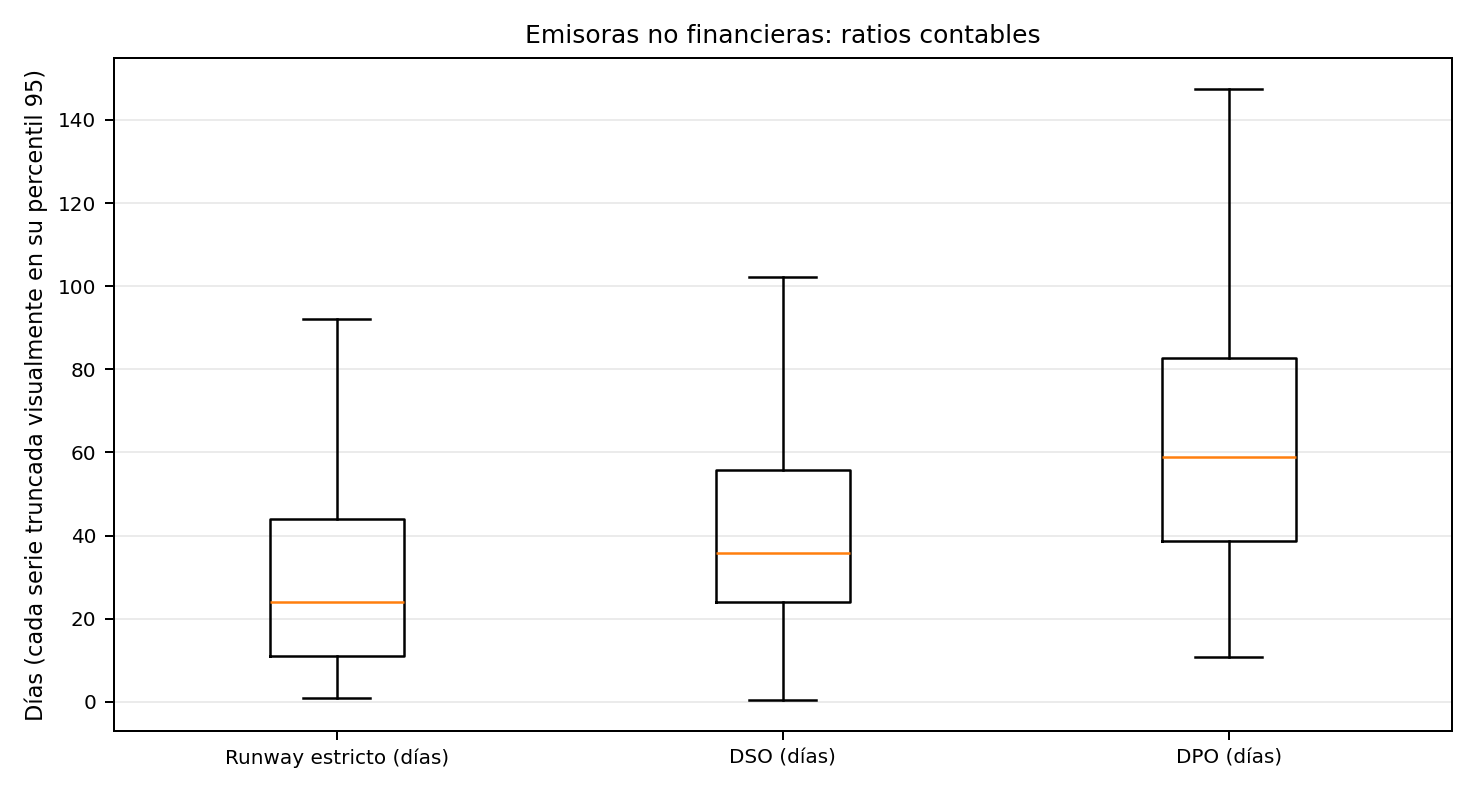
\includegraphics[width=.78\linewidth]{listed_firm_liquidity.png}\caption{Piloto de ratios contables de emisoras argentinas. Las series se truncan visualmente en su percentil 95; la figura es descriptiva, no representativa ni identifica pagos públicos o redes productivas.}\label{fig:pilot}\end{figure}

\section{Endogeneidad, causalidad inversa e identificación}
\subsection{El problema no es un único sesgo}
La relación de interés conecta la demora del pagador público $\tau^g_{it}$, el runway $R_{it}$, la demora propia de la firma a sus proveedores $\delta^s_{it}$, los resultados $Y_{it}$ y la supervivencia $S_{it}$. Son variables distintas: $\tau^g$ mide cuánto tarda el Estado en pagar una obligación a la firma; $\delta^s$ mide cuánto se demora la firma en pagar a sus propios proveedores. Un esquema estructural mínimo es
\begin{align}
R_{it}&=r(\tau^g_{it},C_{it},L^u_{it},B_{it},A^g_{it},Z_{it}),\\
Y_{i,t+1}&=g(R_{it},A_{it},K_{it},N_{it},\varepsilon_{it}),\\
\delta^s_{it}&=d(R_{it},A^p_{it},\text{liquidez}_{it},\text{poder de negociación}_{it},\nu_{it}),\\
\tau^g_{it}&=d(F_{it}^{\mathrm{fiscal}},Q_{it}^{\mathrm{admin}},\text{desempeño contractual}_{it},\zeta_{it}),\\
N_{i,t+1}&=n(N_{it},Y_{it},\delta^s_{it},\xi_{it}),
\end{align}
donde $F^{\mathrm{fiscal}}$ resume restricciones del pagador público, $Q^{\mathrm{admin}}$ la administración contractual, $A^p$ representa las cuentas por cobrar del sector privado y $N$ las relaciones productivas. Esta representación no se estima con los datos disponibles; ordena las fuentes de simultaneidad.

Primero, una demora pública puede causar una brecha de caja que lleve a la firma a retrasar sus propios pagos a proveedores. Segundo, la causalidad inversa puede operar porque problemas de entrega, documentación, calidad o solvencia pueden afectar la certificación de una factura pública, mientras que la fragilidad también puede aumentar $\delta^s$. Tercero, shocks comunes —recesión, inflación, estrés fiscal, cambios regulatorios o condiciones sectoriales— pueden afectar tanto $\tau^g$ como los resultados. Cuarto, la red es endógena: una firma puede cambiar proveedores, concentrar compras o perder clientes como respuesta al mismo shock. Quinto, la selección de muestra es relevante: los estados financieros observan empresas cotizadas que sobreviven hasta reportar; no capturan adecuadamente entradas y salidas del universo empresarial.

La evidencia empírica reciente sobre la demora de las firmas en pagar a sus proveedores enfatiza que ese comportamiento puede reflejar tanto flexibilidad financiera como distress y que los registros de pagos efectivos permiten distinguir patrones que no se recuperan de balances agregados por sí solos \citep{wu2026,hirshleifer2019}. Esta literatura informa el canal de propagación, pero no debe confundirse con evidencia directa sobre la demora del Estado en pagar a sus contratistas. Por eso, una demora no debe interpretarse como tratamiento exógeno ni como indicador unívoco de fragilidad.

\subsection{Estimando y fuentes de no identificación}
El estimando debe elegirse antes de seleccionar un estimador: el efecto total de la demora sobre la supervivencia, el efecto mediado por la liquidez y la respuesta de proveedores expuestos a clientes afectados son objetos distintos. Un coeficiente convencional de panel con efectos fijos de firma y tiempo no identificaría causalidad si la demora pública está correlacionada con shocks no observados, si el desempeño contractual afecta la certificación o el momento de pago, o si los controles incluyen variables posteriores al tratamiento. Los efectos fijos eliminan heterogeneidad invariante en el tiempo, no confusión temporal ni simultaneidad. Controlar por el runway contemporáneo puede bloquear el canal de mediación que se busca estudiar; el error de medición puede introducir sesgos adicionales. Con los datos actuales, el artículo pasa directamente a resultados potenciales y requisitos de diseño, en lugar de presentar una regresión de panel convencional como candidato empírico.

\subsection{Resultados potenciales, exposición de red y estimandos}
Sea $D_i$ la exposición predeterminada a un evento de demora y $Y_i(d,g)$ el resultado de la firma $i$ bajo exposición propia $d$ y exposición de red $g$. Con interferencia, el resultado potencial convencional $Y_i(d)$ es incompleto: también puede depender de si sus clientes o proveedores están expuestos. Un efecto directo a exposición de red fija es $\tau_D(g)=\mathbb E[Y_i(1,g)-Y_i(0,g)]$; un spillover a exposición propia fija es $\tau_G(d)=\mathbb E[Y_i(d,g_1)-Y_i(d,g_0)]$. Son estimandos distintos y requieren un mapa de exposición que resuma las rutas de red relevantes. Si el mapa omite contrapartes importantes, el estimando no queda bien definido para los datos observados.

Una especificación de estudio de eventos podría ser
\begin{equation}
Y_{it}=\alpha_i+\lambda_{st}+\sum_{k\ne-1}\beta_k\,1[t-T_i=k]D_i^0+\sum_{k\ne-1}\gamma_k\,1[t-T_i=k]G_i^0+\varepsilon_{it},
\label{eq:event_study_network}
\end{equation}
donde $D_i^0$ y $G_i^0$ se definen con contratos y enlaces previos al evento, $T_i$ es la fecha del evento, $\alpha_i$ son efectos fijos de firma y $\lambda_{st}$ efectos sector-por-tiempo. Es una plantilla, no una regresión estimada. Su interpretación requiere un evento creíble, ausencia de tendencias diferenciales no tratadas condicionadas al diseño, ausencia de anticipación fuera de la ventana modelada, medición estable y tratamiento defendible de fechas escalonadas y efectos heterogéneos. Si las fechas difieren y los efectos son heterogéneos, un único coeficiente de efectos fijos bidireccionales puede combinar comparaciones con ponderaciones no deseadas; son preferibles estimadores por cohorte y una agregación transparente.

La exposición de red $G_i^0$ debe construirse antes del tratamiento y someterse a sensibilidad respecto del radio, los pesos y la dirección de los enlaces. Un shock directo al contratista público puede transmitirse a proveedores aguas arriba por su comportamiento de pago, mientras que la demora del propio comprador público en pagarle es una exposición diferente. Una misma firma puede ocupar ambas posiciones. No conviene reducirlas a un escalar sin declarar el mapa de exposición. Los errores estándar deben reflejar tanto la asignación del tratamiento como la dependencia de red; puede ser necesario usar inferencia por aleatorización o procedimientos robustos a exposición cuando la agrupación convencional sea insuficiente.

\subsection{Diseño posible, no ejecutado}
Si se documenta una reforma, cambio operativo o regularización que altere plazos de pago de forma plausiblemente exógena, una opción es un estudio de eventos con exposición predeterminada:
\begin{equation}
Y_{it}=\alpha_i+\lambda_t+\sum_{k\neq-1}\beta_k\left(E_i^0\times\1\{t-T^*=k\}\right)+X_{it}'\gamma+u_{it}, \label{eq:eventstudy}
\end{equation}
donde $E_i^0$ es la exposición a compradores públicos medida antes del evento. La interpretación causal requiere ausencia de anticipación, tendencias paralelas condicionales, composición estable o correcciones apropiadas, ausencia de otros shocks diferenciales coincidentes y una definición transparente de exposición. Si el tratamiento se adopta de forma escalonada o los efectos son heterogéneos, deben emplearse estimadores apropiados en lugar de interpretar mecánicamente una regresión convencional de efectos fijos \citep{callaway2021,sun2021,baker2026}.

Una estrategia instrumental necesitaría una variable $Z$ que afecte los plazos de pago, pero no afecte directamente los resultados por otros canales y no esté correlacionada con shocks no observados. Una regla administrativa o una asignación presupuestaria no es un instrumento válido solo por preceder al resultado: puede afectar demanda pública, inversión, calidad de contratación o expectativas. La exclusión y la primera etapa deben defenderse institucionalmente y someterse a pruebas de sensibilidad. No se ha verificado aquí un instrumento que satisfaga esas condiciones.

Para spillovers, la exposición de cada proveedor debe construirse con enlaces anteriores al shock, por ejemplo $E_i^{N,0}=\sum_j W^0_{ij}\tau^g_j$. La inferencia debe admitir interferencia entre unidades: una firma de control puede estar expuesta indirectamente a clientes tratados. Se requieren mapas de exposición explícitos, errores estándar compatibles con el nivel de asignación y pruebas de falsificación en enlaces que no deberían transmitir el shock. El problema de reflexión en modelos de interacción social y la simultaneidad de redes advierten que una correlación entre pares no separa automáticamente influencia de selección o shocks comunes \citep{manski1993,bramoulle2009}.

\begin{table}[htbp]\centering\small
\caption{Amenazas de identificación y respuesta metodológica}
\begin{tabularx}{\linewidth}{p{.23\linewidth}X X}
\toprule
Amenaza & Cómo aparece en este problema & Respuesta necesaria \\
\midrule
Causalidad inversa & La fragilidad puede afectar certificación, puntualidad propia, crédito y condiciones de proveedores & Medir covariables y red antes del shock; establecer el calendario institucional; usar variación exógena defendible \\
Confusión & Estrés fiscal, ciclo sectorial o inflación afectan demoras y resultados & Efectos de tiempo/sector, controles pretratamiento y diseño que justifique comparabilidad \\
Mediación & El runway es un canal entre demora y resultado & Distinguir efecto total de efecto directo; no controlar automáticamente por mediadores \\
Red endógena & La firma cambia de proveedores tras el shock & Congelar exposición pretratamiento y modelar interferencia \\
Selección & Cotizadas y sobrevivientes difieren de entrantes y salientes & Marco muestral empresarial, seguimiento de salida y análisis de selección \\
Error de medición & DSO/DPO y runway no son fechas de factura ni efectivo disponible & Vincular estados, facturas, vencimientos, pagos y crédito comprometido \\
\bottomrule
\end{tabularx}\end{table}

\subsection{Qué evidencia discriminaría los mecanismos}
Una prueba informativa separaría al menos tres grupos definidos antes del shock: firmas con productividad alta y baja liquidez; firmas con productividad y liquidez bajas; y firmas con liquidez suficiente. Si el canal financiero es importante, la respuesta de inversión o supervivencia debería ser más intensa en el primer grupo, siempre que las medidas de productividad y liquidez sean comparables y no estén contaminadas por resultados posteriores. Para separar flexibilidad de distress, hacen falta fechas de pago realizadas, días de atraso respecto del vencimiento, historial de cobranza, acciones de proveedores y resultados posteriores. Los saldos contables por sí solos mezclan atrasos discrecionales y restricciones involuntarias.

La identificación de heterogeneidad no es una solución automática. La exposición predeterminada puede correlacionarse con tamaño, productividad, sector, localización, acceso político, tipo de contrato o tendencias previas. El análisis debe reportar balance, tendencias previas, placebos, sensibilidad a ventanas y definiciones de exposición, y resultados nulos. Si la fuente de variación no supera estas pruebas, el resultado debe permanecer descriptivo.

\subsection{Implicaciones observables, falsación y heterogeneidad}
El marco produce predicciones condicionales que pueden ser refutadas sin imponer que toda demora tenga un efecto negativo. Primero, si la demora reduce efectivamente la fracción monetizable de cuentas por cobrar, el cambio en caja disponible debería concentrarse en firmas con exposición previa relevante y vencimientos cercanos. Una asociación igual de intensa entre firmas sin facturación pública y firmas expuestas sería evidencia contra la interpretación directa, aunque no necesariamente contra otros canales comunes. Segundo, el efecto debería atenuarse cuando existen líneas comprometidas utilizables, reservas líquidas o factoring disponible a costos moderados. Una interacción nula no refuta por sí sola el mecanismo si estas medidas tienen error severo o las líneas se cancelan precisamente durante el shock; obliga, no obstante, a revisar la medición y el supuesto de sustitución financiera.

Tercero, el canal de red implica heterogeneidad según la fracción de ventas expuesta, concentración de clientes, centralidad y posibilidad de sustituir compradores o proveedores. La dirección de transmisión debe definirse antes de estimar: una demora del Estado a la firma contratista y una demora de esa firma a sus proveedores son aristas diferentes, con posibles signos opuestos en balances individuales. El agregado de cuentas por pagar no permite recuperar la matriz de exposiciones ni separar el shock inicial de las respuestas endógenas de proveedores. Cuarto, si la liquidez preserva opciones productivas, las diferencias deberían aparecer en decisiones intermedias —compras, utilización de capacidad, mantenimiento, inversión o innovación— antes que exclusivamente en una productividad agregada de largo plazo. Observar solo supervivencia no permite identificar cuál de esas rutas operó.

La falsación debe incluir resultados que no deberían responder inmediatamente al shock, grupos con exposición previa nula, fechas placebo y medidas alternativas de runway. Los efectos estimados no deberían depender de clasificar como tratamiento la exposición contemporánea, que puede ser una respuesta al propio shock. La heterogeneidad por productividad requiere medir productividad con información anterior al evento y corregir, en la medida posible, el sesgo de supervivencia: la PTF calculada solo entre sobrevivientes no es un resultado neutral a la salida. Cuando las firmas comparten proveedores, la hipótesis de no interferencia entre unidades falla; los errores estándar agrupados por firma no capturan necesariamente shocks comunes en la red. Una inferencia creíble debe definir conglomerados o mapas de exposición que correspondan a la estructura real de dependencia.

Por último, la forma reducida puede distinguir flexibilidad comercial de distress financiero. Si los atrasos permiten suavizar temporalmente caja en relaciones repetidas, algunas firmas pueden retrasar pagos de manera estratégica sin encontrarse al borde de la salida. La misma variable observada —días de demora— puede, por tanto, reflejar un seguro bilateral o una restricción severa. Para separar mecanismos se necesitan vencimiento contractual, fecha efectiva, disputas, penalidades, historial de relación, condiciones de crédito y eventos de incumplimiento. No debe interpretarse el signo de una regresión de días de demora sobre supervivencia sin una estructura que aborde selección y causalidad inversa.

\subsection{Lectura conjunta de los insumos empíricos}
\begin{table}[htbp]\centering\small
\begin{tabularx}{\linewidth}{p{0.17\linewidth}p{0.19\linewidth}p{0.22\linewidth}X}
\toprule
Bloque & Cobertura procesada & Uso válido & No permite afirmar\\
\midrule
Estados contables & 537 informes, 52 emisoras argentinas & Construcción auditada de ratios contables en una muestra seleccionada & Representatividad de todas las firmas o acceso efectivo a crédito/factoring\\
Runway inicial & 44 emisoras no financieras con runway positivo más reciente & Diagnóstico de ajuste de tres cuantiles de la distribución inicial & Identificación estructural de parámetros dinámicos\\
WBES pública & Tablas de frecuencia del catálogo nacional & Contexto descriptivo sobre demoras declaradas y exposición contractual & Microdatos ponderados descargados o efecto causal de los atrasos\\
ABM & Reglas y semillas de escenarios sintéticos & Pruebas de mecanismos bajo una restricción explícita de insumos financiables & Predicción real, equilibrio validado o efecto causal sobre productividad\\
\bottomrule
\end{tabularx}
\caption{Inventario de evidencia y límites de interpretación. Las coberturas describen archivos procesados, no necesariamente el universo estadístico.}\label{tab:evidence_inventory}
\end{table}

El número de filas no es una medida suficiente de calidad de evidencia. Para el piloto contable, el número de informes excede el de emisoras porque hay observaciones repetidas en el tiempo; los errores estándar o resúmenes no deben tratar cada reporte como firma independiente. La auditoría detectó que el archivo supuestamente multi-país era estructuralmente idéntico al argentino; se excluyó del análisis y no se lo considera una muestra separada.

La estadística descriptiva WBES requiere una precaución distinta: un catálogo público o una tabla de frecuencias no equivale a microdatos de establecimientos con pesos, estratos y diseño muestral aplicados. Las frecuencias reportadas pueden motivar hipótesis y ayudar a definir variables, pero no deben usarse para estimar una media nacional ponderada sin reproducir la documentación de muestreo. Tampoco deben combinarse con los estados contables como si compartieran unidad de observación, período o marco muestral.

\section{Diagnóstico computacional y alcance de los resultados}
Los ejercicios numéricos disponibles cumplen funciones distintas. El piloto de emisoras permite evaluar qué ratios pueden construirse con estados contables públicos. El experimento ABM muestra cómo se comporta una parametrización bajo shocks y reglas explícitas. Ninguno identifica el efecto causal de la demora de pagos públicos.

El ajuste parcial del estado inicial modificó la escala y dispersión de la caja para aproximar cuantiles de runway de 44 emisoras no financieras. Los objetivos contables P10, P50 y P90 fueron 4,77, 22,90 y 105,55 días. Sin embargo, en diez semillas nuevas tras 24 períodos, la mediana simulada aumentó a unos 305,95 días y el percentil 90 a 995,17 días. Interpretamos esto no como predicción ni como “descubrimiento” de programación, sino como un experimento de delimitación de frontera: bajo las reglas actuales, la acumulación de liquidez no encuentra contrapesos suficientes en los usos modelados de los excedentes. La ausencia de mecanismos como dividendos contingentes al estado, conversión defensiva de excedentes a moneda extranjera y cancelación o refinanciación forzosa de pasivos financieros es una explicación plausible que debe probarse, no una causa empíricamente establecida. El experimento aísla el canal de acumulación condicionado a las reglas actuales e indica que una calibración futura debe modelar la asignación de excedentes, no solo reajustar los parámetros de los shocks. Por sí solo, no demuestra que las fricciones estándar de la literatura sean insuficientes en general; eso requiere comparar especificaciones alternativas bajo datos y momentos comunes.

El ABM ahora hace depender las ventas realizadas de la proporción de insumos planeados que se financia antes de producir, eliminando la inconsistencia previa entre racionamiento y producción contemporánea. Esta es solo una restricción proporcional estilizada: inventarios, insumos complementarios, utilización de capacidad y precios de insumos no están modelados por completo. Los resultados siguen siendo un ejercicio de mecanismos, no un modelo de red productiva calibrado empíricamente ni una estimación de efectos de las demoras sobre el crecimiento.

El diagnóstico de proyección por bins usa los 44 valores de runway anual seleccionados, expresados en meses, y compara aproximaciones uniformes y por cuantiles para dos integrandos. Los errores muestrales no son monótonos en el número nominal de bins; por ejemplo, la aproximación uniforme de urgencia presenta error absoluto cercano a 0,00004 con 32 bins y aumenta a unos 0,033 con 64 bins. Las cotas Lipschitz uniformes calculadas son amplias. Este ejercicio mide solo la proyección de integrandos sobre una distribución observada; no mide el error del campo vectorial ni certifica convergencia de trayectorias o raíces.

El laboratorio de estados finitos muestra que pueden construirse simulaciones ilustrativas de población abierta y verificar masa no negativa o residuo numérico pequeño. Esas verificaciones son controles de implementación del campo programado. No demuestran que el campo sea una descripción microfundada completa, que la discretización converja globalmente, ni que existan múltiples equilibrios. De manera análoga, una AUC calculada sobre salidas sintéticas evalúa predicción dentro del simulador, no causalidad ni desempeño fuera de muestra sobre empresas reales.

El certificado de Krawczyk documentado para un sistema reducido heredado no se vuelve a ejecutar con independencia en este paquete y no se transfiere al sistema distribucional. La condición de inclusión de una caja solo certifica el objeto matemático al que se aplica. Por eso no se afirma aquí una bifurcación validada, una histéresis general o una irreversibilidad de productividad. Estos resultados requerirían fijar el campo microfundado completo, verificar el cierre del estado, ejecutar continuación de ramas y certificar el sistema concreto.

\section{Agenda futura}
La transición desde proxies contables públicos a microdatos enlazados debe seguir un protocolo preespecificado. Primero, construir una matriz dirigida de pagos $W$ con facturas comprador-proveedor, fijando cada ponderación con promedios de años pretratamiento (y normalizando filas o participaciones de ventas según una regla documentada) para no condicionar mecánicamente la red a cambios contemporáneos al shock. Segundo, definir el tratamiento como un cambio documentado en los plazos de pago de una dependencia pública o provincia y estimar efectos grupo-tiempo con diferencias en diferencias escalonadas, siguiendo a Callaway y Sant’Anna (2021). Deben fijarse de antemano las cohortes, el tiempo relativo al evento, las ventanas de anticipación, los controles aún no tratados, las tendencias previas, las reformas concurrentes y la heterogeneidad; los efectos fijos bidireccionales no deben usarse por defecto cuando la adopción es escalonada. Tercero, enlazar resultados de facturas con runway, demora propia a proveedores, producción, empleo, inversión y salida, separando exposición directa y exposición de red y explicitando los supuestos de interferencia parcial. Cuarto, reportar diagnósticos de estudio de eventos, fechas y resultados placebo, sensibilidad a la definición de red, attrition muestral e inferencia agrupada al nivel de asignación del tratamiento cuando corresponda. El acceso debe ser autorizado y confidencial. Es un protocolo, no una estimación ejecutada; requiere cambios escalonados documentados y grupos de comparación creíbles. En paralelo, la agenda teórica consiste en cerrar el estado mínimo suficiente incluyendo red y pasivos relevantes, validar el campo de dimensión finita y medir por separado error de proyección, error del campo y error de trayectoria. La agenda no presume que estos ejercicios confirmarán el mecanismo: sus criterios de aceptación deben permitir también rechazarlo.

\section{Conclusiones}
La liquidez no crea por sí misma productividad, pero puede determinar cuánto tiempo una firma conserva para sostener pagos, sustituir insumos y convertir oportunidades en producción. En redes productivas, las obligaciones entre firmas hacen posible que una perturbación localizada se propague; el alcance depende de la disponibilidad de crédito, la sustituibilidad y la estructura de los vínculos. Bajo una distribución Lomax, la relación entre runway y riesgo de distress admite una derivación cerrada. Bajo una condición de estabilidad espectral, un modelo lineal local de red admite una representación de propagación no negativa. Y bajo regularidad Lipschitz, la aproximación por bins puede acotarse, siempre que se distinga el error de integración del error del campo y de sus trayectorias.

Estos resultados son condicionales y delimitados. La condición de cierre por momentos exige que las variables omitidas no cambien la transición dentro de una misma fibra de agregación. La demora de pago puede reducir el runway, pero la asociación observada no identifica causalidad si el estrés financiero, la administración contractual, el ciclo económico o la red son endógenos. Los datos actualmente reunidos describen ratios contables de una muestra seleccionada de emisoras; no observan la combinación necesaria de pagos realizados, contrapartes, red, crédito accesible y salida. La discrepancia dinámica del ABM también impide describir su calibración como satisfactoria.

La contribución defendible es, por tanto, una estructura analítica que hace explícitos los mecanismos, las condiciones de validez y los requisitos de identificación. No se afirma que la opcionalidad financiera domine siempre a la productividad ni que la demora pública produzca un efecto causal cuantificado. La hipótesis permanece falsable: con datos transaccionales y una fuente de variación creíble, debe ser posible determinar en qué condiciones la liquidez protege firmas productivas, cuándo los retrasos se propagan y cuándo la sustitución o el financiamiento neutralizan el canal.

\appendix
\section{Demostración de la desigualdad de Jensen para el distress}
Con gasto común $B>0$, escala $s>0$ y forma $\alpha>0$, la función $q_L(R)=(1+BR/s)^{-\alpha}$ satisface $q_L''(R)=\alpha(\alpha+1)(B/s)^2(1+BR/s)^{-\alpha-2}>0$ para todo $R\geq0$. Por tanto, $q_L$ es estrictamente convexa. Como $0<q_L(R)\leq1$, su esperanza existe para cualquier distribución de probabilidad sobre runways no negativos. La desigualdad de Jensen implica $\mathbb E[q_L(R)]\geq q_L(\mathbb E[R])$, con igualdad si y solo si $R$ es constante casi seguramente.

\section{Demostración de la cota de trayectoria}
Sean $x$ y $x_K$ soluciones de $\dot x=F(x)$ y $\dot x_K=F_K(x_K)$ en una región común. Defínase $e(t)=\|x(t)-x_K(t)\|$. Por la representación integral,
\[
e(t)\leq e(0)+\int_0^t\|F(x(s))-F_K(x_K(s))\|\,\dd s.
\]
Sumando y restando $F(x_K(s))$, usando Lipschitz y la cota uniforme del campo,
\[
e(t)\leq e(0)+\int_0^t Le(s)\,\dd s+\int_0^t\delta_K\,\dd s.
\]
La desigualdad de Grönwall produce $e(t)\leq e^{Lt}e(0)+\delta_K(e^{Lt}-1)/L$, que coincide con \eqref{eq:gronwall}. Si $L=0$, la cota límite es $e(t)\leq e(0)+\delta_Kt$.

\section{Demostración del cierre micro--macro distribucional}
Sea $\mathfrak M_t$ el estado completo especificado en el teorema. Por la hipótesis de suficiencia Markoviana, la ley conjunta condicional de decisiones, shocks, indicadores de entrada/salida, elecciones de reconfiguración de red y actualizaciones agregadas, dada la historia $\mathcal F_t=\sigma(\mathfrak M_0,\ldots,\mathfrak M_t)$, depende de $\mathcal F_t$ solo a través de $\mathfrak M_t$. Denótese esa ley por $K(\cdot\mid\mathfrak M_t)$. El siguiente estado completo es una función medible del estado actual y de esos sorteos; su distribución condicional es, por tanto, la imagen de $K$ bajo dicha regla de transición. Defínase esa imagen como $\mathcal P(\cdot\mid\mathfrak M_t)$. Se sigue que $\Pr(\mathfrak M_{t+1}\in A\mid\mathcal F_t)=\mathcal P(A\mid\mathfrak M_t)$ para todo conjunto medible $A$, que es la propiedad Markoviana afirmada. La demostración está condicionada a la hipótesis de suficiencia: no prueba que un modelo empírico particular haya incluido todas las variables de estado relevantes.

\section{Demostración del cierre exacto por momentos}
Sea $X$ el espacio de estados microeconómicos, $S:X\to Y$ el mapa de agregación y $T:X\to X$ la transición. Existe una función $\Phi:S(X)\to Y$ tal que $S(Tx)=\Phi(S(x))$ para todo $x\in X$ si y solo si $S\circ T$ es constante en cada fibra $S^{-1}(y)$.\
\emph{Necesidad.} Si existe $\Phi$ y $S(x_1)=S(x_2)=y$, entonces $S(Tx_1)=\Phi(y)=S(Tx_2)$.

\emph{Suficiencia.} Para cada $y\in S(X)$, elija cualquier $x$ con $S(x)=y$ y defina $\Phi(y)=S(Tx)$. La constancia en la fibra garantiza que esta definición no depende de la elección. Por tanto, el agregado es una estadística de estado suficiente para la transición agregada exactamente cuando microestados con el mismo resumen no divergen en sus agregados siguientes. En sistemas aleatorios, la condición debe formularse para la ley condicional de $S(X_{t+1})$ dado el estado microeconómico, no solo para su media.

\section{Propiedades del multiplicador de red}
Si $W\geq0$ y $\rho(\beta W)<1$, la serie $\sum_{k=0}^{\infty}(\beta W)^k$ converge en norma matricial y coincide con $(I-\beta W)^{-1}$. Para $u\geq0$, cada término $(\beta W)^ku$ es no negativo y, por tanto, $x=(I-\beta W)^{-1}u\geq u$. Si $W$ es reducible, la condición espectral sigue siendo suficiente y la propagación puede quedar confinada a componentes alcanzables desde el shock. Si $\rho(\beta W)\geq1$, no se concluye que las pérdidas económicas diverjan: lo que falla es esta representación lineal estable de rondas infinitas; una dinámica no lineal con salida, sustitución o racionamiento puede estar acotada, pero debe modelarse por separado.

\section{Diccionario mínimo de variables y límites de medición}
\begin{longtable}{>{\raggedright\arraybackslash}p{0.16\linewidth}>{\raggedright\arraybackslash}p{0.25\linewidth}>{\raggedright\arraybackslash}p{0.21\linewidth}>{\raggedright\arraybackslash}p{0.20\linewidth}}
\toprule
Objeto & Construcción conceptual & Fuente disponible & Límite de interpretación\\
\midrule
\endhead
Runway contable & Caja y equivalentes divididos por gasto operativo diario aproximado & Estados contables de emisoras cotizadas & Proxy retrospectivo; no incluye por defecto líneas utilizables, vencimientos diarios ni caja restringida\\
Runway efectivo & Recursos accesibles en horizonte común divididos por obligaciones esenciales & Requiere caja, crédito comprometido, factoring, cuentas por cobrar y vencimientos & No observado de forma completa en los archivos actuales\\
Atraso público & Pago efectivo menos vencimiento contractual, condicionado a exposición previa & No disponible a nivel de factura enlazada & Catálogos y frecuencias públicas no identifican la fecha efectiva para cada factura\\
Atraso comercial & Pago del comprador a proveedor menos vencimiento contractual & No disponible a nivel de relación proveedor-cliente & DPO agregado no recupera el grafo dirigido ni la identidad de la contraparte\\
Exposición de red & Participación de ventas o compras vinculada a cada contraparte antes del shock & No disponible en el panel contable consolidado & No sustituir con grado contemporáneo o sector como si fueran exposición observada\\
Salida de firma & Cese de actividad verificado y fecha de salida & No enlazado en la muestra contable actual & La desaparición de un reporte puede ser falta de cobertura, no salida económica\\
Productividad de firma & Producción o ventas reales con insumos y capital comparables & No disponible para todas las firmas en un panel enlazado & Ratios contables y ventas nominales no identifican productividad física\\
\bottomrule\end{longtable}

La elegibilidad de una variable para regresión debe decidirse antes de estimar y no después de observar el signo del coeficiente. Como mínimo, cada serie requiere un identificador estable, fecha de referencia, unidad, frecuencia, cobertura, definición, regla de transformación y procedencia. La variable se bloquea si una de esas dimensiones críticas no está validada. Los indicadores candidatos extraídos de portales nacionales permanecen como candidatos hasta que se verifique que la etiqueta, la definición estadística y la serie descargada corresponden a la misma magnitud. Un HTTP 200 o un archivo no vacío es una prueba de transporte, no de validez semántica.

\section{Requisitos mínimos de replicación}
Una réplica del análisis empírico debe registrar fuente, fecha de descarga, versión de los metadatos, claves de país y año, unidad, frecuencia, reglas de transformación y hash de cada insumo. Los ratios contables deben conservar los nombres originales de partidas y una tabla de correspondencia auditable. La adquisición de datos de facturas requiere autorización institucional; la ausencia de acceso no debe registrarse como ausencia estructural de datos. Los resultados sintéticos deben guardar semillas, parámetros, versiones de código y reglas de exclusión, y deben etiquetarse como simulaciones.
\subsection{Reproducibilidad Computacional y Disponibilidad de Código}
Para garantizar la transparencia y la falsabilidad empírica de los mecanismos desarrollados en este artículo, el paquete de replicación completo se encuentra disponible públicamente. Este incluye los resolutores analíticos deterministas, los diagnósticos distribucionales de proyección por bins, los scripts de auditoría de microdatos para el piloto de firmas cotizadas argentinas y el código fuente completo del laboratorio de mecanismos basados en agentes. El repositorio documentado, junto con los hashes de integridad de datos y las especificaciones del entorno, está alojado en:
\begin{center}
    \url{https://github.com/brianaxelrodriguez/wealth-of-optionality}
\end{center}
Las pruebas unitarias verifican los invariantes de la restricción de producción bajo racionamiento de capital líquido, pero no certifican la estacionariedad dinámica global ni establecen la identificación estructural de los parámetros.


\begin{thebibliography}{99}
\bibitem[Almeida et al.(2014)]{almeida2014} Almeida, H., Campello, M., Cunha, I. y Weisbach, M. S. (2014). Corporate liquidity management: A conceptual framework and survey. \emph{Annual Review of Financial Economics}, 6, 135--162.
\bibitem[Almeida y Campello(2007)]{almeida2007} Almeida, H. y Campello, M. (2007). Financial constraints, asset tangibility, and corporate investment. \emph{Review of Financial Studies}, 20(5), 1429--1460.
\bibitem[Achdou et al.(2022)]{achdou2022} Achdou, Y., Han, J., Lasry, J.-M., Lions, P.-L. y Moll, B. (2022). Income and wealth distribution in macroeconomics: A continuous-time approach. \emph{Review of Economic Studies}, 89(1), 45--86.
\bibitem[Acemoglu et al.(2012)]{acemoglu2012} Acemoglu, D., Carvalho, V. M., Ozdaglar, A. y Tahbaz-Salehi, A. (2012). The network origins of aggregate fluctuations. \emph{Econometrica}, 80(5), 1977--2016.
\bibitem[Amberg et al.(2021)]{amberg2021} Amberg, N., Jacobson, T., von Schedvin, E. y Townsend, R. (2021). Curbing shocks to corporate liquidity: The role of trade credit. \emph{Journal of Political Economy}, 129(1), 182--242.
\bibitem[Baker et al.(2026)]{baker2026} Baker, A. C., Callaway, B., Cunningham, S., Goodman-Bacon, A. y Sant’Anna, P. H. C. (2026). Difference-in-differences designs: A practitioner’s guide. \emph{Journal of Economic Literature}, 64(2), 498--557.
\bibitem[Barrot y Sauvagnat(2016)]{barrot2016} Barrot, J.-N. y Sauvagnat, J. (2016). Input specificity and the propagation of idiosyncratic shocks in production networks. \emph{Quarterly Journal of Economics}, 131(3), 1543--1592.
\bibitem[Boissay y Gropp(2013)]{boissay2013} Boissay, F. y Gropp, R. (2013). Payment defaults and interfirm liquidity provision. \emph{Review of Finance}, 17(6), 1853--1894.
\bibitem[Bramoullé et al.(2009)]{bramoulle2009} Bramoullé, Y., Djebbari, H. y Fortin, B. (2009). Identification of peer effects through social networks. \emph{Journal of Econometrics}, 150(1), 41--55.
\bibitem[Callaway y Sant’Anna(2021)]{callaway2021} Callaway, B. y Sant’Anna, P. H. C. (2021). Difference-in-differences with multiple time periods. \emph{Journal of Econometrics}, 225(2), 200--230.
\bibitem[Carvalho(2014)]{carvalho2014} Carvalho, V. M. (2014). From micro to macro via production networks. \emph{Journal of Economic Perspectives}, 28(4), 23--48.
\bibitem[Costello(2020)]{costello2020} Costello, A. M. (2020). Credit market disruptions and liquidity spillover effects in the supply chain. \emph{Journal of Political Economy}, 128(9), 3434--3468.
\bibitem[Demir et al.(2024)]{demir2024} Demir, B., Javorcik, B., Michalski, T. K. y Ors, E. (2024). Financial constraints and propagation of shocks in production networks. \emph{Review of Economics and Statistics}, 106(2), 437--454.
\bibitem[Fazzari et al.(1988)]{fazzari1988} Fazzari, S. M., Hubbard, R. G. y Petersen, B. C. (1988). Financing constraints and corporate investment. \emph{Brookings Papers on Economic Activity}, 1988(1), 141--206.
\bibitem[Gourieroux et al.(1993)]{gourieroux1993} Gourieroux, C., Monfort, A. y Renault, E. (1993). Indirect inference. \emph{Journal of Applied Econometrics}, 8(S1), S85--S118.
\bibitem[Hirshleifer et al.(2019)]{hirshleifer2019} Hirshleifer, D., Li, Y., Lourie, B. y Ruchti, T. (2019, revisado en 2023). Do trade creditors possess private information? Stock returns evidence. NBER Working Paper 25553.
\bibitem[Hopenhayn(1992)]{hopenhayn1992} Hopenhayn, H. A. (1992). Entry, exit, and firm dynamics in long run equilibrium. \emph{Econometrica}, 60(5), 1127--1150.
\bibitem[Huremović et al.(2026)]{huremovic2026} Huremović, K., Jiménez, G., Moral-Benito, E., Peydró, J.-L. y Vega-Redondo, F. (2026). Production and financial networks in interplay. \emph{American Economic Review}, 116(5), 1611--1647.
\bibitem[Jacobson y von Schedvin(2015)]{jacobson2015} Jacobson, T. y von Schedvin, E. (2015). Trade credit and the propagation of corporate failure: An empirical analysis. \emph{Econometrica}, 83(4), 1315--1371.
\bibitem[Jovanovic(1982)]{jovanovic1982} Jovanovic, B. (1982). Selection and the evolution of industry. \emph{Econometrica}, 50(3), 649--670.
\bibitem[Krusell y Smith(1998)]{krusell1998} Krusell, P. y Smith, A. A. (1998). Income and wealth heterogeneity in the macroeconomy. \emph{Journal of Political Economy}, 106(5), 867--896.
\bibitem[Manski(1993)]{manski1993} Manski, C. F. (1993). Identification of endogenous social effects: The reflection problem. \emph{Review of Economic Studies}, 60(3), 531--542.
\bibitem[Melitz(2003)]{melitz2003} Melitz, M. J. (2003). The impact of trade on intra-industry reallocations and aggregate industry productivity. \emph{Econometrica}, 71(6), 1695--1725.
\bibitem[Solow(1957)]{solow1957} Solow, R. M. (1957). Technical change and the aggregate production function. \emph{Review of Economics and Statistics}, 39(3), 312--320.
\bibitem[Sun y Abraham(2021)]{sun2021} Sun, L. y Abraham, S. (2021). Estimating dynamic treatment effects in event studies with heterogeneous treatment effects. \emph{Journal of Econometrics}, 225(2), 175--199.
\bibitem[World Bank Group(2026)]{wbes2026} World Bank Group. (2026). Argentina: Enterprise Survey 2025. Catálogo y documentación pública de la encuesta. \url{https://microdata.worldbank.org/catalog/8489}.
\bibitem[Wu et al.(2026)]{wu2026} Wu, J., Lee, H.-H. y Birge, J. R. (2026). The hidden world of trade credit: The flexibility role of late payments. \emph{Journal of Supply Chain Management}. Publicado en línea el 18 de agosto de 2026. doi:10.1177/10591478261480286.
\end{thebibliography}
\end{document}
